\documentclass[11pt,border=2mm,tikz]{standalone}
\usepackage{csquotes}
\usepackage[backend=biber,style=numeric,sorting=none]{biblatex}

\providecommand{\FigScale}{0.92}

\usepackage{siunitx}
\usepackage{tikz}
\usetikzlibrary{decorations.pathmorphing, patterns, arrows.meta, calc}
\usetikzlibrary{shapes.geometric, arrows}
\usetikzlibrary{positioning}
 
\usepackage{amsmath}
 
\usepackage{tikz-3dplot}
\usetikzlibrary{3d}
 
\usepackage[siunitx,american]{circuitikz}
 
\usepackage{pgfplots}
\usepgfplotslibrary{units}
\usepgfplotslibrary{groupplots}
\pgfplotsset{compat=1.14}
 
\ctikzset{tripoles/mos style/arrows}



\definecolor{IBM4}{HTML}{fe6100}%orange - sensor
\definecolor{IBM5}{HTML}{ffb000}%gul - end device/module
\definecolor{IBM8}{HTML}{0072b2}%blågrøn
\definecolor{IBM10}{HTML}{009e73}%grøn - PCB

\begin{document}
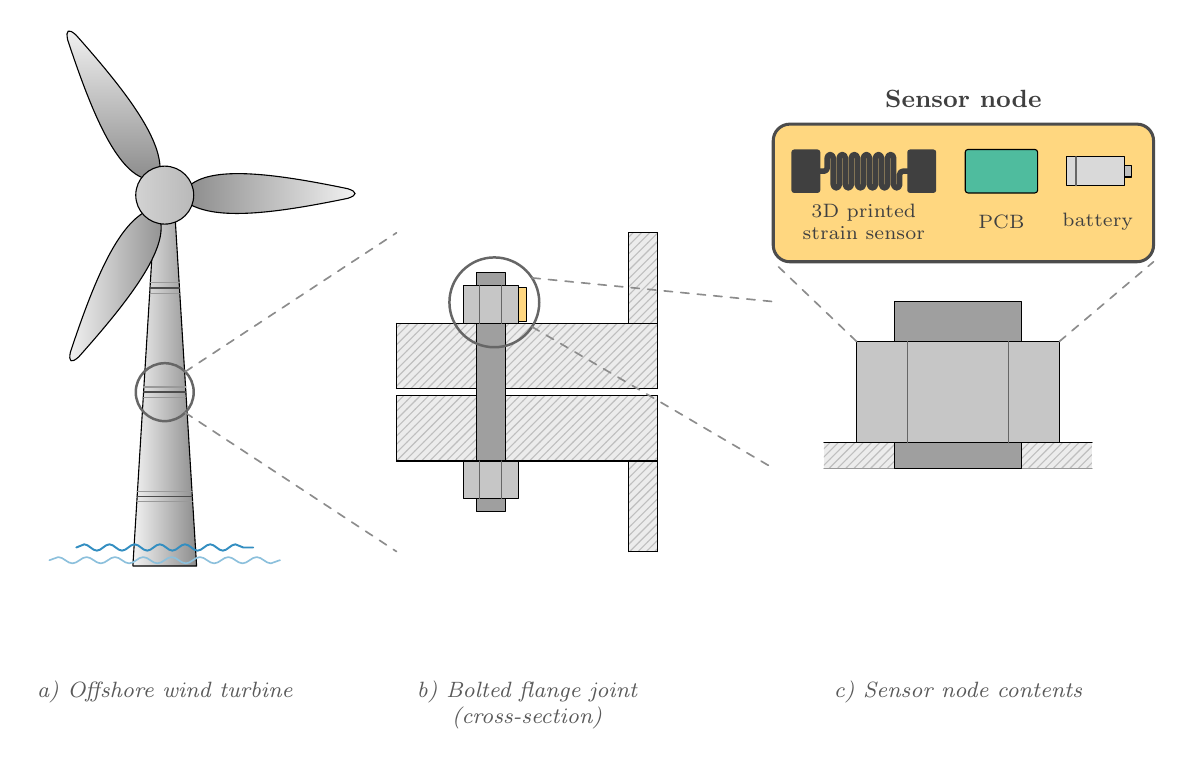
\begin{tikzpicture}[
  scale=\FigScale,
  line join=round, line cap=round,
  zoomline/.style={dashed, black!45, line width=0.6pt},
  zoomcircle/.style={black!60, line width=0.9pt},
  lbl/.style={font=\scriptsize, text=black!75, align=center},
  leader/.style={black!50, line width=0.5pt},
  panelcap/.style={font=\footnotesize\itshape, text=black!65, align=center}
]

\begin{scope}[shift={(2.5,1.1)}, scale=0.8]
  \path[shade, left color=gray!10, right color=gray!90, draw=black]
    (-0.55,0) -- (0.55,0) -- (0.18,6) -- (-0.18,6) -- (-0.55,0);
  \foreach \fy/\fw in {1.2/0.476, 3/0.365, 4.8/0.254} {
    \draw[black!70, line width=0.5pt] (-\fw,\fy) -- (\fw,\fy);
    \draw[black!40, line width=0.4pt] (-\fw,\fy+0.09) -- (\fw,\fy+0.09);
    \draw[black!40, line width=0.4pt] (-\fw,\fy-0.09) -- (\fw,\fy-0.09);
  }
  \def\bladeScale{0.69}
  \begin{scope}[rotate around={30:(0,6.4)}]
    \begin{scope}[shift={(0,6.8)}, scale=\bladeScale, shift={(0,-6.8)}]
      \path[shade, top color=gray!10, bottom color=gray!90, draw=black]
        (0.2,6.8)
        .. controls (0.65,7.51) and (0.45,9.00) .. (0.08,10.8)
        .. controls (0.0,11.04) and (-0.08,11.04) .. (-0.16,10.8)
        .. controls (-0.55,8.92) and (-0.75,7.35) .. (-0.2,6.8) -- (0.2,6.8);
    \end{scope}
  \end{scope}
  \begin{scope}[rotate around={150:(0,6.4)}]
    \begin{scope}[shift={(0,6.8)}, scale=\bladeScale, shift={(0,-6.8)}]
      \path[shade, left color=gray!10, right color=gray!90, draw=black]
        (0.2,6.8)
        .. controls (0.65,7.51) and (0.45,9.00) .. (0.08,10.8)
        .. controls (0.0,11.04) and (-0.08,11.04) .. (-0.16,10.8)
        .. controls (-0.55,8.92) and (-0.75,7.35) .. (-0.2,6.8) -- (0.2,6.8);
    \end{scope}
  \end{scope}
  \begin{scope}[rotate around={270:(0,6.4)}]
    \begin{scope}[shift={(0,6.8)}, scale=\bladeScale, shift={(0,-6.8)}]
      \path[shade, right color=gray!10, left color=gray!90, draw=black]
        (0.2,6.8)
        .. controls (0.65,7.51) and (0.45,9.00) .. (0.08,10.8)
        .. controls (0.0,11.04) and (-0.08,11.04) .. (-0.16,10.8)
        .. controls (-0.55,8.92) and (-0.75,7.35) .. (-0.2,6.8) -- (0.2,6.8);
    \end{scope}
  \end{scope}
  \path[shade, left color=gray!35, right color=gray!55, draw=black] (0,6.4) circle (0.5);

  \draw[decorate, decoration={snake, amplitude=0.4mm, segment length=3.2mm},
        IBM8!80, line width=0.7pt] (-1.525,0.32) -- (1.525,0.32);
  \draw[decorate, decoration={snake, amplitude=0.4mm, segment length=3.6mm},
        IBM8!45, line width=0.6pt] (-1.99,0.1) -- (1.99,0.1);

  \draw[zoomcircle] (0,3) circle (0.5);
  \coordinate (zA1) at ($(0,3)+(45:0.5)$);
  \coordinate (zA2) at ($(0,3)+(-45:0.5)$);
\end{scope}



\draw[zoomline] (zA1) -- (5.7,5.7);
\draw[zoomline] (zA2) -- (5.7,1.3);

\fill[gray!15] (5.7,3.55) rectangle (9.3,4.45);
\fill[gray!15] (8.9,4.45) rectangle (9.3,5.7);
\fill[gray!15] (5.7,2.55) rectangle (9.3,3.45);
\fill[gray!15] (8.9,1.3)  rectangle (9.3,2.55);
\draw[pattern=north east lines, pattern color=black!25]
  (5.7,3.55) rectangle (9.3,4.45);
\draw[pattern=north east lines, pattern color=black!25]
  (8.9,4.45) rectangle (9.3,5.7);
\draw[pattern=north east lines, pattern color=black!25]
  (5.7,2.55) rectangle (9.3,3.45);
\draw[pattern=north east lines, pattern color=black!25]
  (8.9,1.3) rectangle (9.3,2.55);
\draw[black] (5.7,4.45) -- (9.3,4.45) (5.7,3.55) -- (9.3,3.55)
             (5.7,3.45) -- (9.3,3.45) (5.7,2.55) -- (9.3,2.55)
             (5.7,3.55) -- (5.7,4.45) (5.7,2.55) -- (5.7,3.45)
             (9.3,2.55) -- (9.3,3.45) (9.3,3.55) -- (9.3,4.45);
\draw[black] (8.9,4.45) -- (8.9,5.7) (9.3,4.45) -- (9.3,5.7)
             (8.9,1.3) -- (8.9,2.55) (9.3,1.3) -- (9.3,2.55);

\fill[gray!75, draw=black] (6.8,1.85) rectangle (7.2,5.15);
\fill[gray!45, draw=black] (6.62,4.45) rectangle (7.38,4.97);
\draw[black!60, line width=0.4pt] (6.85,4.45) -- (6.85,4.97)
                                  (7.15,4.45) -- (7.15,4.97);
\fill[gray!45, draw=black] (6.62,2.03) rectangle (7.38,2.55);
\draw[black!60, line width=0.4pt] (6.85,2.03) -- (6.85,2.55)
                                  (7.15,2.03) -- (7.15,2.55);

\fill[IBM5!50, draw=black] (7.38,4.48) rectangle (7.5,4.94);

\draw[zoomcircle] (7.05,4.74) circle (0.62);
\coordinate (zB1) at ($(7.05,4.74)+(33:0.62)$);
\coordinate (zB2) at ($(7.05,4.74)+(-33:0.62)$);



\draw[zoomline] (zB1) -- (10.9,4.75);
\draw[zoomline] (zB2) -- (10.9,2.45);

\begin{scope}[shift={(0,0.9)}]

\fill[gray!15] (11.6,1.55) rectangle (15.3,1.9);
\fill[pattern=north east lines, pattern color=black!25] (11.6,1.55) rectangle (15.3,1.9);
\draw[black] (11.6,1.9) -- (15.3,1.9);
\draw[black!40, line width=0.4pt] (11.6,1.55) -- (15.3,1.55);
\fill[gray!75, draw=black] (12.575,1.55) rectangle (14.325,3.85);
\fill[gray!45, draw=black] (12.05,1.9) rectangle (14.85,3.3);
\draw[black!60, line width=0.4pt] (12.75,1.9) -- (12.75,3.3)
                                  (14.15,1.9) -- (14.15,3.3);

\draw[zoomline] (12.05,3.3) -- (10.9,4.4);
\draw[zoomline] (14.85,3.3) -- (16.15,4.4);

\begin{scope}[shift={(0,0.25)}]

\draw[black!70, line width=1.1pt, rounded corners=6pt, fill=IBM5!50]
  (10.9,4.15) rectangle (16.15,6.05);
\node[anchor=center, font=\small\bfseries, text=black!75] at (13.525,6.4) {Sensor node};

\begin{scope}[shift={(-0.075,0.25)}]
\def\sensorturns{13}
\def\sensorlinewidth{2pt}
\pgfmathsetmacro{\sensordx}{1.0/(\sensorturns-1)}
\pgfmathsetmacro{\sensorrad}{0.49*\sensordx}
\pgfmathtruncatemacro{\sensorpenult}{\sensorturns-1}
\draw[black!75, line width=\sensorlinewidth, rounded corners={\sensorrad cm}]
  (11.5,5.15) -- (11.72,5.15) -- (11.72,5.38)
  \foreach \i in {2,...,\sensorpenult} {
    -- ({11.72+(\i-1)*\sensordx}, {isodd(\i-1) ? 5.38 : 4.92})
    -- ({11.72+(\i-1)*\sensordx}, {isodd(\i) ? 5.38 : 4.92})
  }
  -- (12.72, {isodd(\sensorpenult) ? 5.38 : 4.92})
  -- (12.72,5.15) -- (12.95,5.15);
\end{scope}

\fill[black!75, rounded corners=1pt] (11.15,5.1) rectangle (11.55,5.7);
\fill[black!75, rounded corners=1pt] (12.75,5.1) rectangle (13.15,5.7);
  
\node[lbl] at (12.15,4.7) {3D printed\\ strain sensor};

\fill[IBM10!69, draw=black, rounded corners=1pt] (13.55,5.1) rectangle (14.55,5.7);
\node[lbl] at (14.05,4.7) {PCB};

\fill[gray!30, draw=black] (14.95,5.2) rectangle (15.75,5.6);
\fill[gray!50, draw=black] (15.75,5.32) rectangle (15.84,5.48);
\draw[black!60, line width=0.4pt] (15.08,5.2) -- (15.08,5.6);
\node[lbl] at (15.38,4.7) {battery};
\end{scope}

\end{scope}



\node[panelcap, anchor=north] at (2.5,-0.35)  {a) Offshore wind turbine};
\node[panelcap, anchor=north] at (7.5,-0.35)  {b) Bolted flange joint\\ (cross-section)};
\node[panelcap, anchor=north] at (13.45,-0.35) {c) Sensor node contents};

\end{tikzpicture}
\end{document}
